\renewcommand{\LangOO}{\ensuremath{{\mathcal{L}}_{ul}}\xspace }

\section{The Underlying Programming Language \LangOO}  
\label{sect:underlying}

\subsection{\LangOO syntax and runtime configurations}
\label{sub:Loo} 
This work is based on \LangOO, a {minimal}, imperative, sequential,  class based, typed, object-oriented language. 
We believe, however, that the work can easily be adapted to any capability safe language with some form of encapsulation,
and that it can also support inter-language security, provided that the 
platform offers means to protect a module’s private state; cf capability-safe hardware as in Cheri \cite{davis2019cheriabi}.
Wrt to encapsulation and  capability safety,  \LangOO supports private fields, private and public methods, unforgeable addresses, and no ambient authority (no static methods, no address manipulation).
To reduce the complexity of our formal models, as is usually done, \eg \cite{IgaPieWadTOPLAS01,DietlDrossopoulouMueller07a,ParBiePOPL05},  \LangOO lacks many common languages features, omitting static fields and methods, interfaces,
inheritance, subsumption, exceptions, and control flow.  
{In our examples, we use numbers and booleans -- these can be encoded.}
 
Fig. \ref{f:loo-syntax} shows the   \LangOO syntax. {Statements, $stmt$, are three-address instructions,   method calls, or empty, $\epsilon$.}  
Expressions, $\re$, are ghost code;  as such, they may appear in assertions but not in statements, and have no side-effects \cite{ghost,ghost:spirit}.
Expressions  may contain fields, $\re.f$, or ghost-fields, ${\re_0.gf(\overline {\re})}$.
The meaning of $\re$ is module-dependent; \eg$\prg{a}.\prg{\balance}$   is a field lookup  in \ModA , but in a module which stores balances in a table it would be a recursive lookup through that table  -- \cf example   in \S \aref{A.3 }{app:BankAccount:ghost}. 
  \footnote
{For convenience,   $\re.gf$ is short for $\re.gf()$. Thus,  $\re.gf$ may be simple field lookup  in some modules, or  ghost-field  in others. }
In line with most tools, we support ghost-fields, but they are not central to our work.
 

\LangOO states, $\sigma$,  consist of a  heap $\chi$ and a stack. 
{A stack  is a sequence of frames, $\phi_1\!\cdot\!...\!\cdot\! \phi_n$.}
A  frame, $\phi$, consists of a local variable map and a continuation, \ie {the}  
statements to be executed.
The top frame, \ie  the frame most recently pushed onto the stack,  in a state $(\phi_1\!\cdot\!...\!\cdot\! \phi_n, \chi)$ is $\phi_n$.



\begin{figure}[t]
\footnotesize{
$
 \begin{array}{ll}
 \begin{syntax}
\syntaxElement{Mdl}{Module Def.}
		{
		\syntaxline{\overline{C\ \mapsto\ CDef}}\endsyntaxline
		}
\endSyntaxElement\\
\syntaxElement{CDef}{Class Def.}
		{
		% [An]\
		 \prg{class}\ C\ 
		\{\  \overline{fld}; \overline{mth};\  \overline{gfld};\  \}		
		}
\endSyntaxElement 
\\
\syntaxElement{mth}{Method Def.}
		{
		\syntaxline
		{ {p}\  \prg{method}\ m\ (\overline{x : T}){:T}\{\ s\ \} }
		\endsyntaxline
		}
\endSyntaxElement
\end{syntax}
 &    
\begin{syntax}
\syntaxElement{fld}{Field Def.}
		{\syntaxline
			{\prg{field}\ f\ :\ T}
		\endsyntaxline}
\endSyntaxElement 
\\
\syntaxElement{T}{Type}
		{
		\syntaxline
				{C}
		\endsyntaxline
		}
\endSyntaxElement
\\
\syntaxElement{p}{Privacy}
		{
		\syntaxline
		{\prg{private}}
		{\prg{public}}
		\endsyntaxline
		}
\endSyntaxElement 
\end{syntax}

 \end{array}
 $
\\
\[
\begin{syntax}
\syntaxElement{stmt}{ } %Statements
		{
				\syntaxline
				{{x:=y}}
				{{x:=v}}
				{x:=y.f}
				{x.f:=y}
				{x:=y_0.m(\overline{y})}
				{x:=\prg{new} \ {C} }
				{ stmt;\ stmt }
				  { \epsilon }
			       \endsyntaxline
		}
\endSyntaxElement
\\
\syntaxElement{gfld}{Ghosts}
		{\syntaxline
			{\prg{ghost}\ gf(\overline{x : T})\{\ \re\ \} : T}
%			{\prg{ghost}\ \prg{intrnl}\ g\  (\overline{x : T})\{\ gt\ \} : T} -- DO NOT REMOVE THESE yet
		\endsyntaxline}
\endSyntaxElement\\
\syntaxElement{{\re}}{{{ }}} %Expr
		{
		\syntaxline
				{x}
				{v}
				{\re.f}
				{{\re.gf(\overline {\re})}}
		\endsyntaxline
		}
\endSyntaxElement
\\
\end{syntax}
\]
\\
 $
 \begin{array}{lcl}
 \begin{syntax}
\syntaxElement{\sigma}{Program {State}}
		{
		\syntaxline
		{( \overline \phi, \chi )}
		\endsyntaxline
		}
\endSyntaxElement 
\\
\syntaxElement{\phi}{Frame}
		{
		\syntaxline
		{  (\  \overline{x\mapsto v};\ s \ ) }
		\endsyntaxline
		}
\endSyntaxElement\\
\syntaxElement{\chi}{Heap}
		{(\  \overline{\alpha \mapsto o}\ )}
\endSyntaxElement
\end{syntax}
 & \hspace{1cm} & 
\begin{syntax}
\syntaxElement{{C, f, m, gf, x, y}}{ }
		{{Identifier}}
\endSyntaxElement\\
\syntaxElement{o}{Object}
		{(\ C;\  \overline{f \mapsto v} \ )}
\endSyntaxElement\\
\syntaxElement{v}{Value}
		{
		\syntaxline
				{\alpha} % {i}	{\true} 	{\false} -- DO NOT REMOVE THESE yet
				{\nul}
		\endsyntaxline
		}
\endSyntaxElement
\end{syntax}

 \end{array}
 $
 }
\caption{\LangOO Syntax. We use $x$, $y$, $z$ for variables, \ $C$, $D$ for class identifiers, $f$ for field identifier, ${gf}$ for ghost field identifiers, $m$ for method identifiers, $\alpha$ for addresses.
%, $i$ for integers.
}
\label{f:loo-syntax}
\end{figure}


 
 
\paragraphsd{Notation.} We adopt the following unsurprising notation:
\label{s:notation}
\begin{itemize}
\item
{An object is uniquely identified by the address that points to it. We shall be talking of objects $o$, $o'$ when talking less formally, and of addresses, $\alpha$, $\alpha'$, $\alpha_1$, ...  when more formal.}
\item
$x$, $x'$, $y$, $z$, $u$, $v$, $\va$  are {variables}; \ 
% \item
$dom(\phi)$ and $Rng(\phi)$ indicate the variable map in $\phi$; \ \ $dom(\sigma)$ and $Rng(\sigma)$ indicate the variable map in the top frame in $\sigma$
\item
$\alpha \in \sigma$ means that $\alpha$ is defined in the heap of $\sigma$, and $x\in \sigma$ means that $x\in dom(\sigma)$.
Conversely,  $\alpha\notin\sigma$ and $x\notin\sigma$ %, and $\va \notin A$ h
 have the obvious meanings.
$\interpret{\sigma}{\alpha}$  is $\alpha$; and $\interpret{\sigma}{x}$  is the value to which  $x$  is mapped in the top-most frame of $\sigma$'s stack, 
and $\interpret{\sigma}{e.f}$ looks up in $\sigma$'s heap the value of $f$ for the object  $\interpret{\sigma}{e}$.
% too much detail?
% Note that $\interpret{\sigma}{e}$ is not defined when $e$ contains a method call or a ghost field.
\item %The  update
$\phi[x \mapsto \alpha]$ updates  the variable map  of $\phi$,  
and  $\sigma[x \mapsto \alpha]$ updates the top frame of $\sigma$. \
% \item
$A[\re/x]$ is textual substitution where we replace all occurrences of $x$ in $A$ by $\re$. 
\item
As usual, $\overline q$ stands for  sequence $q_1$, ... $q_n$, where $q$ can be an address, a variable,    a frame, an update or a substitution.
Thus,   $\sigma[\overline{x \mapsto \alpha}]$ and $A[ \overline{e/y}]$ 
% applies the substitutions $\overline{x \mapsto \alpha}$ to the top frame.
have the expected meaning.
\item
$\phi.\prg{cont}$ is the continuation of frame $\phi$, and  $\sigma.\prg{cont}$ is the continuation in the top frame.
\item
$text_1 \txteq text_2$ expresses that $text_1$ and $text_2$ are  the same text.%textually equal.
% the below moved to appendix
%  $s_1 \txtin   s_2$  means  $s_1 \txteq  s_2$ or  $s_2 \txteq  s_1; s_3$ for some $s_3$, where $s_1$, $s_2$, and $s_3$ are program statements. 
\item
We define the depth of a stack as $\DepthFs {\phi_1...\phi_n} \triangleq n$. For states, $\DepthSt {(\overline \phi, \chi)} \triangleq  \DepthFs {\overline \phi}$.
The  operator $\RestictTo  \sigma k$ truncates the stack up to the $k$-th frame: % from $\sigma$. Namely, 
 $\RestictTo {(\phi_1...\phi_k...\phi_n,\chi)} {k}  \triangleq   (\phi_1...\phi_k,\chi)$
\item
{ $\vs(stmt)$ returns the variables which appear in $stmt$. For example, $\vs(u:=y.f)$=$\{u,y\}$.}
\end{itemize}

  

  
\subsection{\LangOO Execution}
\label{sect:execution}

{Fig. \ref{f:loo-semantics} describes \LangOO execution}  by a small steps operational semantics with shape  $\leadstoOrig  {\Mtwo} {\sigma}   {\sigma'}$.
  $\Mtwo$ stands for one or more modules, where a
  module,  $M$, maps class names to class definitions. 
  {%We use the functions 
  The functions $\class{\sigma}{x}$, $\meth{\Mtwo}{C}{m}$,
  { $fields(\Mtwo,C)$,}
    $\Same {x} {y} {\sigma}{\Mtwo}$, and $\Formals {\sigma}  {\Mtwo}$,
return the class of $x$, the method $m$ for class $C$, {the fields for class $C$,} whether $x$ and $y$ belong to the same module, and 
 the formal parameters of the method currently executing in $\sigma$ -- \cf Defs
\aref{A.2 -- A.7}{\ref{def:class-lookup} -- \ref{def:params}}. %  \ref{def:meth-lookup}, \ref{{def:fields-lookup}, \ref{def:same:module}, and  \ref{def:params}.
Initial states, $\initial{\sigma}$, contain a single frame 
with single variable \prg{this} pointing to a single object 
in the heap % of class \prg{Object}, 
and a continuation, \cf \aref{A.8}{def:initial}.
}

\begin{figure}[bt]
\begin{minipage}{\textwidth}
\footnotesize{
\begin{mathpar}
\infer
	{
	{\sigma.\prg{cont}  \txteq  x := y.f; stmt} \ \ \ \ \ \ \ 
	 x \notin \Formals {\sigma} {\Mtwo} \\  
	 \Same {\prg{this}}  {y}  {\sigma} {\Mtwo}
	 % \\
	% \sigma_2=\sigma_1[x\mapsto  \interpret{\sigma_1}{y.f} \} ][\prg{cont} \mapsto stmt ] 
	}
	{\exec{\Mtwo}{\sigma}{\sigma[x\mapsto  \interpret{\sigma}{y.f} \} ][\prg{cont} \mapsto stmt ] }}
	\quad(\textsc{Read})
	\and
\infer
	{
	\sigma .\prg{cont}  \txteq  x.f := y; stmt \ \ \ \ \ \ \ 
	%  x \notin \Formals {\sigma} {\Mtwo} \\
	\Same {\prg{this}}  {x}  {\sigma} {\Mtwo} 
% \\	\sigma_2 = \sigma_1[\interpret{\sigma_1}{x}.f \mapsto\ \interpret{\sigma_1}{y} ][\prg{cont}\mapsto s]	
	}
	{\exec{\Mtwo}{\sigma}{\sigma[\interpret{\sigma}{x}.f \mapsto\ \interpret{\sigma}{y} ][\prg{cont}\mapsto stmt]}}
	{}
	\quad(\textsc{Write})
	\and
\infer
	{
	\sigma.\prg{cont}\  \txteq\  x := {\prg{new}\ C }; stmt \ \ \ \ \ \ \ 
	 x \notin \Formals {\sigma} {\Mtwo} \\ 
	\textit{fields}(\Mtwo,C)=\overline{f} \\
	% {\overline v}   \mbox{ initial values for } \overline f\\
	\alpha \mbox{ fresh in } \sigma
	% \\
        % \sigma_2 = \sigma_1[x\mapsto \alpha][\alpha  \mapsto  (\ C;\  \overline{f\, \mapsto \, v} \  ] [\prg{cont}\mapsto s] 		
	}
	{\exec{\Mtwo}{\sigma}{\sigma[x\mapsto \alpha][\alpha  \mapsto  (\ C;\  \overline{f\, \mapsto \, \nul} \  ) ] [\prg{cont}\mapsto stmt] }}
	\quad(\textsc{New})
\and
\infer
	{
	   {\phi_n}.\prg{cont}  \txteq   u := y_0.m(\overline{y}); \_ \ \ \ \ \ \ \ 
	   u \notin \Formals {( {\overline{\phi}\cdot\phi_n},  \chi)} {\Mtwo} 	   \\
    \meth{\Mtwo}{\class{(\phi_n,\chi)}{y_0}}{m} = p \ C\!::\!m(\overline{x : T}){:T}\{\, stmt\, \}\ \ \ \\
        	{{p=\prg{public}  \vee   \Same{\prg{this}} {y_0} {(\phi_n,\chi)}{\Mtwo} }} 
	% \\
%	\phi_{n+1}= {  (\  \prg{this}\, \mapsto\, \interpret{\phi_n}{y_0},\overline{x\, \mapsto\, \interpret{\phi_n}{y}}; \ stmt\ ) } 
	}
	{\exec{\Mtwo}{ ( {\overline{\phi}\cdot\phi_n},  \chi) }{{(\overline{\phi}\cdot\phi_n\cdot(\  \prg{this}\, \mapsto\, \interpret{\phi_n}{y_0},\overline{x\, \mapsto\, \interpret{\phi_n}{y}}; \ stmt\ )},\chi)}}
	\quad(\textsc{Call})
	\and
\infer
	{
		\phi_{n+1}.\prg{cont} \txteq  {\epsilon} \\  
	\phi_n.\prg{cont}   \txteq  {x := y_0.m(\overline y)}; stmt  
	% \\ \phi'_n= \phi[x \mapsto \interpret{\phi_{n+1}}{\prg{res}}][\prg{cont} \mapsto {stmt} ]
			}
	{\exec{\Mtwo}{({\overline{\phi} \cdot \phi_n \cdot \phi_{n+1}}, \chi) }{({\overline{\phi}\cdot \phi_{n}[x \mapsto \interpret{\phi_{n+1}}{\prg{res}}][\prg{cont} \mapsto {stmt} ]}, \chi)}}
	\quad(\textsc{Return})
\end{mathpar}
 }
\end{minipage}
% \vspace{-0.4cm}
 \caption{\LangOO operational Semantics}
\label{f:loo-semantics}
\end{figure}

The semantics is unsurprising:  
The  top frame's continuation {(${\sigma.\prg{cont}}$)} contains the statement to be  executed next.  
We dynamically enforce a simple form of module-wide privacy: 
Fields may be read or written only if they {belong to an object (here $y$)} whose class comes from the same module as the  class of the object 
%whose field is being read or written, and the class of the object which is 
reading or writing the fields ($\prg{this}$). \footnote{More fine-grained privacy, \eg C++ private fields or ownership types, would provide all
the guarantees needed in our work.} % belong to the same module. 
Wlog, {to simplify some proofs} we  require, as in Kotlin, that method bodies do not assign to formal parameters.

Private methods may be called only if the class of %the receiver (
the callee ({the object whose method  is being called -- here $y_0$}) % ), and the class of the caller (the object which is calling) belong to the same module.
comes from the same module as the  class of the caller (here $\prg{this}$).
Public methods may always be called.
% Statements may assign to variables, allocate new objects,  perform field reads and writes on objects, and call methods on those objects. 
When a method is called, a new frame is pushed onto the stack; this frame  maps \prg{this} and the formal parameters to  the values for the receiver and other arguments, and the continuation to the body of the method. 
Method bodies are expected to store their return values in the {implicitly defined} variable \prg{res}\footnote{For ease of presentation, we omit assignment to \prg{res} in methods returning \prg{void}.}. % in  the examples in this paper \prg{void} methods omit the assignment to \prg{res}.}
  When the continuation is  empty ($\epsilon$), the frame is popped and the value of \prg{res}
 from the popped frame  is stored  in the variable map of the top frame.

{Thus, when $\leadstoOrig {\Mtwo}{\sigma}   {\sigma'} $ is within the same method we have  $\DepthSt {\sigma'}$= $\DepthSt {\sigma}$;\  when it is a call we have
 $\DepthSt {\sigma'}$= $\DepthSt {\sigma}+1$; \ and when it is a return we have  $\DepthSt {\sigma'}$= $\DepthSt {\sigma}-1$.}
Fig. \ref{fig:illusrPreserve}  from \S \ref{s:outline} % \ref{fig:UpSemantics}
distinguishes % illustrates  % such 
  ${\leadstoN}$ {execution} steps into: %. We distinguish
steps within the same  call ($\rightarrow$),\   entering a method  ($\uparrow$),\    returning from a method  ($\downarrow$).
%Thus,  $\sigma_8 \rightarrow \sigma_9$ indicates that  
Therefore $\leadstoOrig {\Mtwo}{\sigma_8}   {\sigma_9} $ is a step within the same call, 
%\ $\sigma_9 \uparrow \sigma_{10}$ indicates that 
$\leadstoOrig {\Mtwo}{\sigma_9}   {\sigma_{10}} $ is a method entry with $\leadstoOrig {\Mtwo}{\sigma_{12}}   {\sigma_{13}} $
% \ with   $\sigma_{12} \downarrow \sigma_{13}$   
the corresponding return. 
In general,  $\leadstoOrigStar  {\Mtwo} {\sigma}   {\sigma'}$ may involve {any}  number of  calls or returns: \eg
% $\leadstoOrigStar  {\Mtwo} {\sigma_8}   {\sigma_{12}}$ involves one call and no return, while 
$\leadstoOrigStar  {\Mtwo} {\sigma_{10}}   {\sigma_{15}}$,   involves no calls and two returns.


%\begin{figure}[htb]
%\begin{tabular}{|c|}
% \hline %  \\ -- this added one vertical space
%\resizebox{7cm}{!}{
%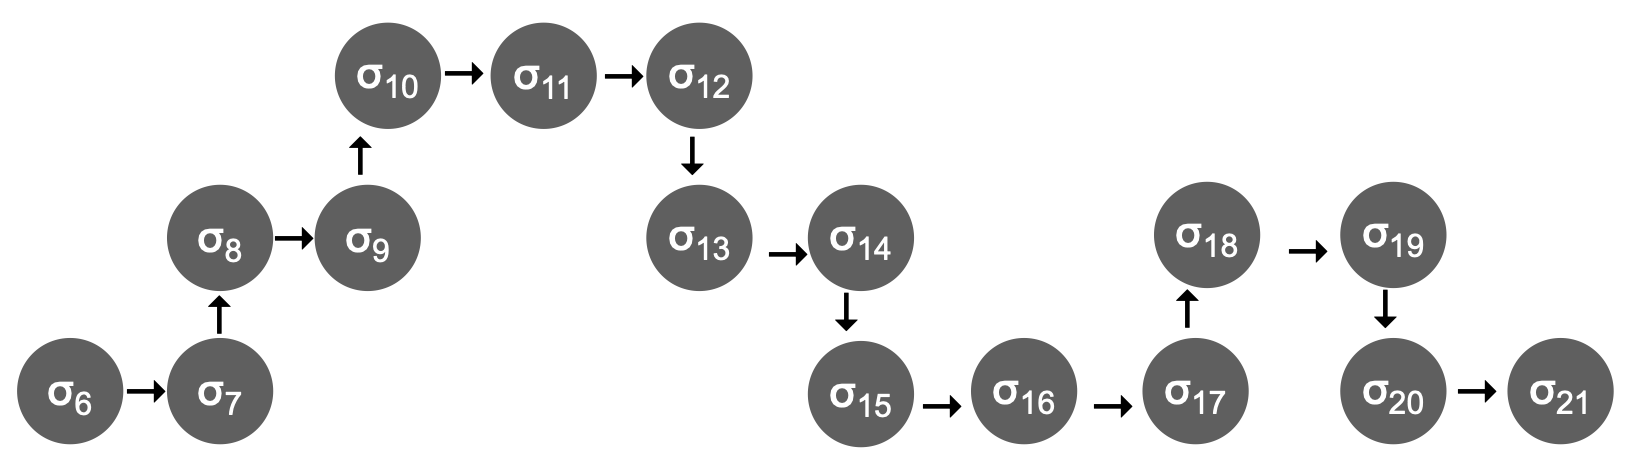
\includegraphics[width=\linewidth]{diagrams/bounded2.png}
%} 
% \\
%\hline
%
%\end{tabular}
%   \caption{$\rightarrow$:\  step within the same method; \ \ $\uparrow$:\    entering a method;\ \  $\downarrow$:  returning from a method}
%   \label{fig:UpSemantics}
% \end{figure}
 

\subsection{Fundamental  Concepts}
\label{s:auxiliary}

The novel features of our assertions — protection and scoped invariants  
— are both defined in terms of the current point of execution.
Therefore, for the semantics of our   assertions we need to represent calls and returns, scoped execution, and (in)directly accessible objects.
 
 \subsubsection{Method Calls and Returns} These  are characterized through pushing/popping   frames :
$ \PushSF  {\phi} {\sigma}$ pushes 
frame $\phi$ onto the stack of $\sigma$, while
% the  operator 
${\sigma\, \popSymbol}$   pops the top frame % of $\sigma$'s stack -- SD dropped as obvious,
and updates the continuation and variable map.

 
 
%\forget{
%\begin{definition}
%\label{def:push:frame}
%Given a state $\sigma$, addresses $\overline \alpha$, a frame $\phi$,  variables or addresses $\overline \va$, we define
%\begin{itemize}
%\item
% $ \PushSF  {\phi} {\sigma} \ \triangleq \ ({\overline{\phi}\cdot\phi}, \chi)$ \ \ \  if \ \ \  $\sigma=(\overline{\phi}, \chi)$.
%\item
%$ \ \sigma\, \popSymbol \ \ \  \triangleq\   { (\overline{\phi}\cdot (\phi_n[\prg{cont}\mapsto stmt][x \mapsto \interpret {\phi_n}{ret}]), \chi)}$ \ \ \  if \\
% $\strut \hspace{1.2cm}  \exists x, y_0, \overline y. [ \ \sigma=(\overline{\phi}\cdot\phi_n\cdot\phi_{n+1}, \chi)$, and $\phi_n(\prg{cont})\txteq x:= y_0.m(\overline y); stmt \ ]$
%\end{itemize}
% \end{definition}
% }
 
 
\begin{definition}
\label{def:push:frame}
Given a state $\sigma$, and a frame $\phi$,  we define
\begin{itemize}
\item
 $ \PushSF  {\phi} {\sigma} \ \triangleq \ ({\overline{\phi}\cdot\phi}, \chi)$ \ \ \  if \ \ \  $\sigma=(\overline{\phi}, \chi)$.
\item
$ \ \sigma\, \popSymbol \ \ \  \triangleq\   { (\overline{\phi}\cdot (\phi_n[\prg{cont}\mapsto stmt][x \mapsto \interpret {\phi_n}{\prg{res}}]), \chi)}$ \ \ \  if \\
 $\strut \hspace{1.5cm} \sigma=(\overline{\phi}\cdot\phi_n\cdot\phi_{n+1}, \chi)$, and $\phi_n(\prg{cont})\txteq x:= y_0.m(\overline y); stmt $
\end{itemize}
 \end{definition}

 \noindent Consider Fig. \ref{fig:illusrPreserve}  again: $\sigma_8 = \PushSF  {\phi} {\sigma_7}$ for some $\phi$, {and}  $\sigma_{15}$=$\sigma_{14} \popSymbol$.
%SD dropped terms called state and callee state
%--  thus $\sigma_8$ is a {\emph{called}} state for 
% $\sigma_7$, and  $\sigma_{15}$ is the {\emph{return}} state from 
% $\sigma_{14}$.

 
 \subsubsection{Scoped Execution}
 \label{sect:bounded}


In order to give semantics to scoped invariants (introduced in \S  \ref{sect:approach:scoped} and to be fully defined  in Def.  \ref{def:necessity-semantics}), we need a new definition of execution, called \emph{scoped execution}. 

 
 \renewcommand{\EarlierS}[2]{\DepthSt{#1} \leq \DepthSt{#2}}
 \renewcommand{\NotEarlierS}[2]{\DepthSt{#1} \not\leq \DepthSt{#2}} 
 
\begin{definition}[Scoped Execution] Given modules $\Mtwo$, and states $\sigma$, $\sigma_1$, $\sigma_n$, and $\sigma'$, we define:
\label{def:shallow:term}
 
\begin{itemize}

  \item
{  $\leadstoBounded  {\Mtwo} {\sigma}   {\sigma'} \ \ \   \,   \ \ \ \triangleq \ \ \  \leadstoOrig {\Mtwo} {\sigma} {\sigma'} \, \wedge\, 
 \EarlierS {\sigma}  {\sigma'} $}
  \item
{  $\leadstoBoundedStar {\Mtwo}  {\sigma_1}  {\sigma_n}  \ \ \,  \ \    \ \triangleq  \ \ \  {\sigma_1} = {\sigma_n}\ \ \vee \ \  \exists \sigma_2,...\sigma_{n-1}.\forall i\!\in\! [1..n)[\  \leadstoOrig {\Mtwo}  {\sigma_i}  {\sigma_{i+1}}\  \wedge\  \EarlierS{\sigma_1} {\sigma_{i+1}} \ ]$ }
% \wedge\,  \EarlierS{\sigma_1} {\sigma_n}$}\ \  
\item
  $\leadstoBoundedStarFin {\Mtwo}  {\sigma}  {\sigma'}  \  \,  \ \  \ \triangleq  \ \ \  \leadstoBoundedStar {\Mtwo}  {\sigma}  {\sigma'}  \ \wedge\ \
 {\DepthFs \sigma = \DepthFs {\sigma'} \ \ \wedge \ \ \sigma'.\prg{cont}=\epsilon  } $
 \end{itemize}
\end{definition}


Consider    Fig. \ref{fig:illusrPreserve} :
Here $\EarlierS {\sigma_8} {\sigma_9}$
and thus $\leadstoBounded   {\Mtwo} {\sigma_8} {\sigma_9}$.
Also,  $\leadstoOrig {\Mtwo} {\sigma_{14}}  {\sigma_{15}}$  \
  but  $\NotEarlierS {\sigma_{14}} {\sigma_{15}} $
  (this step returns from the active call in $\sigma_{14}$),
  and hence   $\notLeadstoBounded  {\Mtwo}  {\sigma_{14}}   {\sigma_{15}}$. 
Finally, even though $\DepthSt {\sigma_8} = \DepthSt {\sigma_{18}}$
%$\sigma_8$ and $\sigma_{18}$ have the same depth of stack 
 and $\leadstoOrigStar {\Mtwo} {\sigma_8}  {\sigma_{18}}$, we have  
 $\notLeadstoBoundedStar {\Mtwo} {\sigma_8}   {\sigma_{18}}$:
This is so, because the execution $\leadstoOrigStar {\Mtwo} {\sigma_8}  {\sigma_{18}}$ goes through the step
$\leadstoOrig {\Mtwo} {\sigma_{14}}  {\sigma_{15}}$ and  $\NotEarlierS {\sigma_{8}} {\sigma_{15}} $
 (this step returns from the active call in  $\sigma_8$).

\vspace{.1cm}
{The relation $\boundedTrans$ contains more than the transitive closure of  $\bounded$.
\Eg, ${\leadstoBoundedStar  {\Mtwo}  {\sigma_9}  {\sigma_{13}}}$, even though ${\leadstoBounded   {\Mtwo}  {\sigma_{9}}  {\sigma_{12}}}$  and ${\notLeadstoBoundedStar   {\Mtwo}  {\sigma_{12}}  {\sigma_{13}}}$.} 
%
Lemma \ref{l:params:do:not:change} says that the value of the parameters does not change during  execution of the same method. 
Appendix \aref{B}{\ref{app:aux}} discusses proofs, and further properties.% of scoped execution, 
 

%Lemma \ref{lemma:orig:to:bounded:front} says  that \scoped executions describe the same set of executions as those  starting at an initial state\footnote{An \emph{Initial} state's heap contains a single object of class \prg{Object}, and
%its  stack   consists of a single frame, whose local variable map is a mapping from \prg{this} to the single object, and whose continuation is   statement.
%(See Def. \ref{def:initial})}. 
%{Lemma \ref{l:var:unaffect} says that scoped execution does not affect the contents of variables in earlier frames.}
%and that 
%the interpretation of a variable remains unaffected by
%scoped execution of statements  which do not mention that variable.


\begin{lemma}
\label{l:params:do:not:change} 
 
For all $\Mtwo$, $\sigma$, $\sigma'$:
 $\strut \hspace{0.3cm} \leadstoBoundedStar {\Mtwo}  {\sigma}  {\sigma'} \ \wedge  \ \DepthFs{\sigma}=\DepthFs {\sigma'}\ \ \ \Longrightarrow\ \  \ \forall x\in \Formals {\Mtwo} {\sigma}.[ \ \interpret \sigma x = \interpret {\sigma'} x \ ]$

\end{lemma}
 






\subsubsection{Reachable  Objects, Locally Reachable Objects, and Well-formed States}

To define protection (no external object indirectly accessible from the top frame
has access to the protected object, \cf \S~\ref{sect:approach:protection}) we first define
reachability. %  and state well-formedness.
%  
%%  {A central concept to our work is %object 
%% protection, \se{that no locally reachable external object can have %unmitigated
%% \se{direct} access to that object}. We define it formally in  Sect. \ref{sect:protect}}
%
An object
% $\alpha'$ is  \emph{reachable} from another object $\alpha$, i.e., $\alpha' \in  \Relevant \alpha   \sigma $, if there is path from $\alpha$ to $\alpha'$; and 
$\alpha$ is
 \emph{locally reachable}, i.e. $\alpha \in  \LRelevantO   \sigma $, if it is reachable from the top frame on the stack of $\sigma$.
 
\begin{definition} We define 
\begin{itemize}
\item
{{$\Relevant {\alpha} {\sigma}  \ \ \ \ \ \triangleq \ \  \  \{ \ \alpha' \, \mid \ \exists n\!\in\!\mathbb{N}.\exists f_1,...f_n. [\ \interpret {\sigma} {\alpha.f_1...f_n} = \alpha'\ ] \ \}$}}.
\item
$ \LRelevantO   \sigma  \ \  \ \triangleq \ \  \  \{ \ \alpha \ \mid \ { \exists x\in dom(\sigma) \wedge \alpha \in \Relevant {\interpret  {\sigma} x}
{\sigma} \ \} } $.
% \exists n\!\in\!\mathbb{N}.\exists f_1,...f_n, x. [\ \interpret {\sigma} {x.f_1...f_n} = \alpha\ ]$}
\end{itemize}
\end{definition}

% \subsection{Well-formed states}

 
In well-formed states, $\Mtwo \models \sigma$,    the value of a parameter in  any callee   (${\RestictTo  \sigma {k}}$) is also the %same as the 
 value of some variable in the caller (${\RestictTo  \sigma {k\!-\!1}}$),
and any address reachable from any frame (${\LRelevantO   {\RestictTo  \sigma {k}} }$) is reachable from some formal parameter of that frame. 
 


\begin{definition}[Well-formed states]
\label{def:wf:state}
 For modules $\Mtwo$, and  states $\sigma$, $\sigma'$:

$\Mtwo \models \sigma \ \ \triangleq \ \  \forall k\in \mathbb{N}. [ \  1<k\leq \DepthFs {\sigma} \ \Longrightarrow $\\
$\strut \hspace{2.25cm}[\ \ \forall   x \in   \Formals {\RestictTo  \sigma {k}} {\Mtwo}.[\ \exists y. \ \interpret {\RestictTo  \sigma {k}}  {x} = \interpret {\RestictTo  \sigma {k\!-\!1}}  {y} \ ]$ $\hspace{0.3cm} \ \ \  \wedge$  
% $\strut \hspace{2.5cm} \ \ \  \wedge$
\\
$\strut \hspace{2.5cm}  {\LRelevantO   {\RestictTo  \sigma {k}} } = \bigcup_{z \in {\Formals {\RestictTo  {\sigma} {k}} {\Mtwo}}}  
{\Relevant { \interpret   {\RestictTo  \sigma {k}}  {z}}\sigma }  \  \ \ \ \ \ ] $
% \ \ \forall \alpha\!\in\! {\LRelevantO   {\RestictTo  \sigma {k}} }.\exists  z\!\in\!  \Formals {\RestictTo  {\sigma} {k}} {\Mtwo}. \alpha\in \Relevant { \interpret   {\RestictTo  \sigma {k}}  {z}}\sigma  \  \ ] \ \ \ \ ] $ 
\end{definition}
 
 
 
Lemma  \ref{lemma:relevant} % describes properties of global reachability. 
says that 
(\ref{wf:preserve}) execution preserves well-formedness, and 
(\ref{oneLR}) any object which is locally reachable after pushing a frame was locally reachable before pushing that frame.
%, and 
 
\begin{lemma}
\label{lemma:relevant}
\label{l:wf:state}
\label{lemma:push:N}
For all modules $\Mtwo$, states $\sigma$, $\sigma'$,   and frame $\phi$:
\begin{enumerate}
\item
\label{wf:preserve}
$\Mtwo \models \sigma \ \wedge \ {\exec{\Mtwo} {\sigma} {\sigma'}}  \ \    \Longrightarrow \ \ \Mtwo \models \sigma' $
\item
\label{oneLR}
{$ \sigma'= \PushSF {\phi} {\sigma}   \ \wedge  \   \Mtwo \models \sigma' %  {Rng(\phi)} \subseteq \LRelevantO  {\sigma} 
 \ \  \Longrightarrow\ \ \LRelevantO {\sigma'}\  \subseteq \LRelevantO   {\sigma}$}

\end{enumerate}
\end{lemma}

 
 
  
  
  
%\footnote{A stronger lemma can be proven:
%% Lemma \ref{lemma:push:N:S} says that % $\pushSymbol$ characterizes  calls and returns. 
%\  (\ref{pushOne}):\  If $\leadstoOrig {\Mtwo} {\sigma}   {\sigma'} $ and $\sigma'\!\in\!\PushS   {\alpha} {\sigma}$ then $\sigma'$ is a  \emph{called} state of $\sigma$ --  {a direct successor state of    $\sigma$  after calling a method}. % with receiver and arguments $\overline \alpha$): \ 
%$\sigma'\in   \PushS  {\alpha} {\sigma}  \ \ \Longleftrightarrow \ \ 
%\exists x, m.[\ \ \sigma.\prg{cont} \txteq x:=y_0.m(y_1,..y_n); \_\ \ \wedge \ \overline \alpha = \overline{ \interpret \sigma y} \ \ ] $
%\\
% (\ref{pushTwo}):\  If $\leadstoOrig {\Mtwo} {\sigma}   {\sigma'} $ and $\sigma\! \in\! \PushS   {\alpha} {\sigma'}$  then $\sigma'$ is a  \emph{caller} state  of $\sigma$ -- {a direct successor  of $\sigma$}  after returning from a method:
% \ \ 
% $\sigma\in   \PushS  {\alpha} {\sigma'}  \ \ \Longleftrightarrow \ \ \exists x, \alpha'.[\ \  \sigma.\prg{cont}\txteq\alpha' \ \ \wedge \ \ \sigma'.\prg{cont}\txteq x:=\alpha';\_ \ \ ] $
% }
  

